\documentclass{article}
\usepackage{tikz}
\usetikzlibrary{decorations.pathreplacing}
\usepackage{amsmath}

\begin{document}

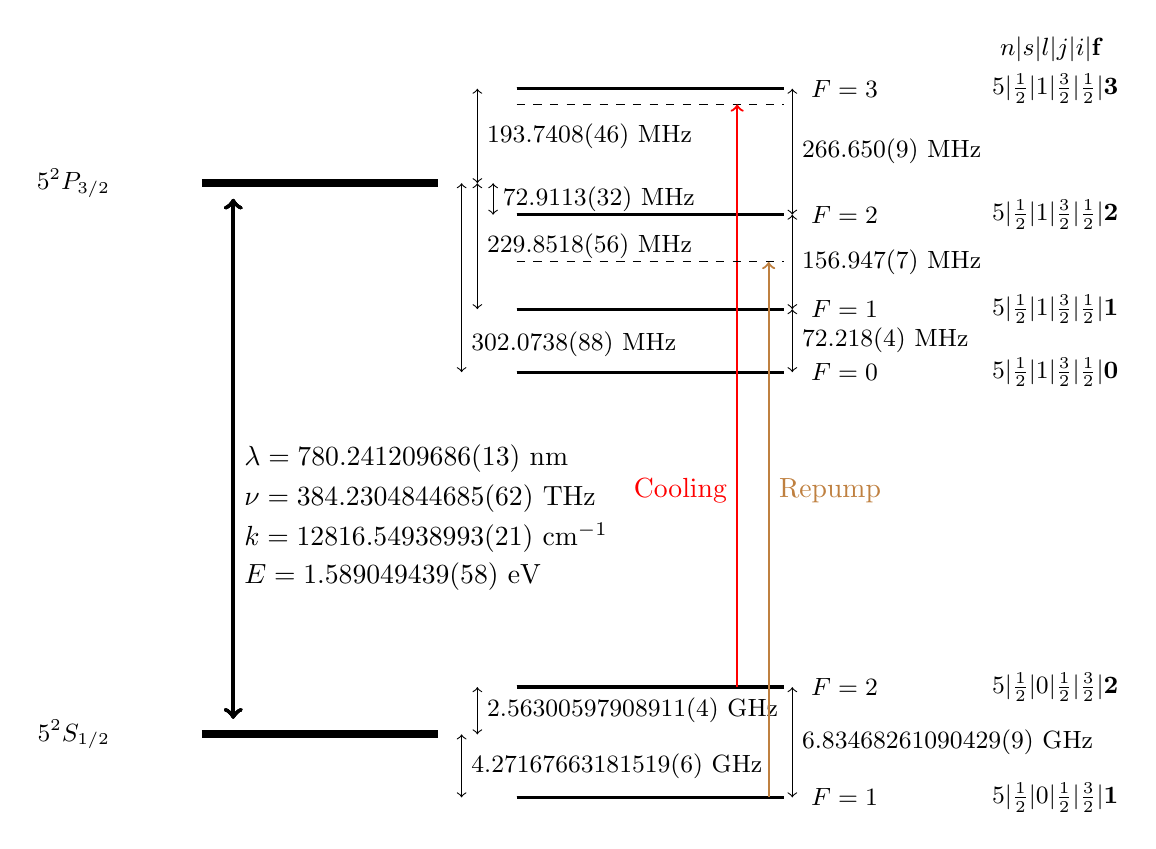
\begin{tikzpicture}[scale=2]

% lower level: 5s 1/2
\draw[line width=1mm] (-2.5,0) -- (-1,0) node[left, xshift=-4cm] {\small $5^2S_{1/2}$};
\draw[very thick] (-0.5,0.3) -- (1.2,0.3) node[right, xshift = 0.2cm] {\small $F = 2$};
\draw[very thick] (-0.5,-0.4) -- (1.2,-0.4) node[right, xshift = 0.2cm] {\small $F = 1$};

\draw[very thick] (-0.5,0.3) -- (1.2,0.3) node[right, xshift = 2.5cm] {\small $5 | \frac{1}{2} | 0 | \frac{1}{2} | \frac{3}{2} | \textbf{2}$};
\draw[very thick] (-0.5,-0.4) -- (1.2,-0.4) node[right, xshift = 2.5cm] {\small $5 | \frac{1}{2} | 0 | \frac{1}{2} | \frac{3}{2} | \textbf{1}$};

% annotate hfs for 5s: F=1 to F=2
\draw[<->] (1.25,0.3) -- (1.25,-0.4) node[midway,right] {\small $6.83468261090429(9)~\text{GHz}$}; % 1 to 2

% annotate hfs for 5s: ground state to F=1,2
\draw[<->] (-0.85,0) -- (-0.85,-0.4) node[midway,right] {\small $4.27167663181519(6)~\text{GHz}$}; % to 1
\draw[<->] (-0.75,0) -- (-0.75,0.3) node[midway,right] {\small $2.56300597908911(4)~\text{GHz}$}; % to 2


% upper level: 5p 3/2
\draw[line width=1mm] (-2.5,3.5) -- (-1,3.5) node[left, xshift=-4cm] {\small $5^2P_{3/2}$};

\draw[very thick] (-0.5,4.1) -- (1.2,4.1) node[right, xshift = 0.2cm] {\small $F = 3$};
\draw[very thick] (-0.5,3.3) -- (1.2,3.3) node[right, xshift = 0.2cm] {\small $F = 2$};
\draw[very thick] (-0.5,2.7) -- (1.2,2.7) node[right, xshift = 0.2cm] {\small $F = 1$};
\draw[very thick] (-0.5,2.3) -- (1.2,2.3) node[right, xshift = 0.2cm] {\small $F = 0$};


\draw[very thick] (-0.5,4.1) -- (1.2,4.1) node[right, xshift = 2.6cm, yshift = 0.5cm] {\small $n | s | l | j | i | \textbf{f}$}; % extra annotation
\draw[very thick] (-0.5,4.1) -- (1.2,4.1) node[right, xshift = 2.5cm] {\small $5 | \frac{1}{2} | 1 | \frac{3}{2} | \frac{1}{2} | \textbf{3}$};
\draw[very thick] (-0.5,3.3) -- (1.2,3.3) node[right, xshift = 2.5cm] {\small $5 | \frac{1}{2} | 1 | \frac{3}{2} | \frac{1}{2} | \textbf{2}$};
\draw[very thick] (-0.5,2.7) -- (1.2,2.7) node[right, xshift = 2.5cm] {\small $5 | \frac{1}{2} | 1 | \frac{3}{2} | \frac{1}{2} | \textbf{1}$};
\draw[very thick] (-0.5,2.3) -- (1.2,2.3) node[right, xshift = 2.5cm] {\small $5 | \frac{1}{2} | 1 | \frac{3}{2} | \frac{1}{2} | \textbf{0}$};

% annotate hfs for 5p: each F state to other F state 
\draw[<->] (1.25,2.3) -- (1.25,2.7) node[midway,right] {\small $72.218(4)~\text{MHz}$}; %0 to 1
\draw[<->] (1.25,2.7) -- (1.25,3.3) node[midway,right] {\small $156.947(7)~\text{MHz}$}; % 1 to 2
\draw[<->] (1.25,3.3) -- (1.25,4.1) node[midway,right] {\small $266.650(9)~\text{MHz}$}; % 2 to 3

% annotate hfs for 5p: ground state to each F state 
\draw[<->] (-0.85,3.5) -- (-0.85,2.3) node[below, right, yshift = 0.35cm] {\small $302.0738(88)~\text{MHz}$};
\draw[<->] (-0.75,3.5) -- (-0.75,2.7) node[midway,right] {\small $229.8518(56)~\text{MHz}$};
\draw[<->] (-0.65,3.5) -- (-0.65,3.3) node[midway,right] {\small $72.9113(32)~\text{MHz}$};
\draw[<->] (-0.75,3.5) -- (-0.75,4.1) node[midway,right] {\small $193.7408(46)~\text{MHz}$};


% cooling transition
\draw[dashed] (-0.5,4.0) -- (1.2,4.0) node[right] {};
% \draw[->,thick, color = red] (1,0.3) -- (1,4.0) node[midway, left, xshift=-0.2cm] {\small $780.241~\text{nm}$};
\draw[->,thick, color = red] (0.9,0.3) -- (0.9,4.0) node[midway, left, yshift = -1.2cm] {Cooling};


% repump transition
\draw[dashed] (-0.5,3.0) -- (1.2,3.0) node[right] {};
% \draw[->,thick, color = red] (1,0.3) -- (1,4.0) node[midway, left, xshift=-0.2cm] {\small $780.241~\text{nm}$};
\draw[->,thick, color = brown] (1.1,-0.4) -- (1.1,3.0) node[midway, right, yshift = 0.5cm] {Repump};



% annotate fs info
\draw[<->, line width = 0.5mm] (-2.3,0.1) -- (-2.3,3.4) node[midway,right, yshift = 0.0cm] {$\lambda = 780.241209686(13)~\text{nm}$};
\draw[<->, line width = 0.5mm] (-2.3,0.1) -- (-2.3,3.4) node[midway,right, yshift = -0.5cm] {$\nu = 384.2304844685(62)~\text{THz}$};
\draw[<->, line width = 0.5mm] (-2.3,0.1) -- (-2.3,3.4) node[midway,right, yshift = -1.0cm] {$k = 12816.54938993(21)~\text{cm$^{-1}$}$};
\draw[<->, line width = 0.5mm] (-2.3,0.1) -- (-2.3,3.4) node[midway,right, yshift = -1.5cm] {$E = 1.589049439(58)~\text{eV}$};



% \node at (1,-0.7) {\small $\lambda = 780.241209686(13)~\text{nm}$};
% \node at (1,-0.9) {\small $\nu = 384.2304844685(62)~\text{THz}$};
% \node at (1,-1.1) {\small $E = 1.589049439(58)~\text{eV}$};

\end{tikzpicture}

\end{document}





















\documentclass{article}
\usepackage{tikz}
\usetikzlibrary{decorations.pathreplacing}
\usepackage{amsmath}

\begin{document}

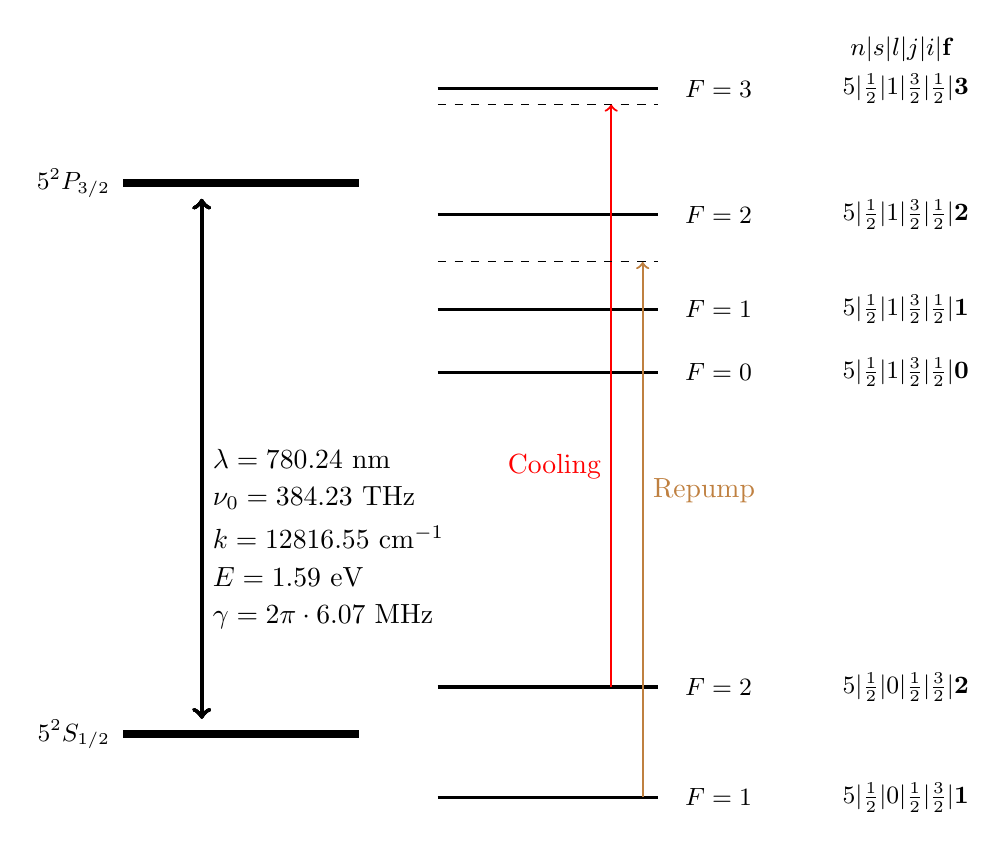
\begin{tikzpicture}[scale=2]

% lower level: 5s 1/2
\draw[line width=1mm] (-2.5,0) -- (-1,0) node[left, xshift=-3cm] {\small $5^2S_{1/2}$};
\draw[very thick] (-0.5,0.3) -- (0.9,0.3) node[right, xshift = 0.2cm] {\small $F = 2$};
\draw[very thick] (-0.5,-0.4) -- (0.9,-0.4) node[right, xshift = 0.2cm] {\small $F = 1$};

\draw[very thick] (-0.5,0.3) -- (0.9,0.3) node[right, xshift = 2.2cm] {\small $5 | \frac{1}{2} | 0 | \frac{1}{2} | \frac{3}{2} | \textbf{2}$};
\draw[very thick] (-0.5,-0.4) -- (0.9,-0.4) node[right, xshift = 2.2cm] {\small $5 | \frac{1}{2} | 0 | \frac{1}{2} | \frac{3}{2} | \textbf{1}$};

% % annotate hfs for 5s: F=1 to F=2
% \draw[<->] (0.95,0.3) -- (0.95,-0.4) node[midway,right] {\small $6.83~\text{GHz}$}; % 1 to 2

% % annotate hfs for 5s: ground state to F=1,2
% \draw[<->] (-0.85,0) -- (-0.85,-0.4) node[midway,right] {\small $4.27~\text{GHz}$}; % to 1
% \draw[<->] (-0.75,0) -- (-0.75,0.3) node[midway,right] {\small $2.56~\text{GHz}$}; % to 2


% upper level: 5p 3/2
\draw[line width=1mm] (-2.5,3.5) -- (-1,3.5) node[left, xshift=-3cm] {\small $5^2P_{3/2}$};

\draw[very thick] (-0.5,4.1) -- (0.9,4.1) node[right, xshift = 0.2cm] {\small $F = 3$};
\draw[very thick] (-0.5,3.3) -- (0.9,3.3) node[right, xshift = 0.2cm] {\small $F = 2$};
\draw[very thick] (-0.5,2.7) -- (0.9,2.7) node[right, xshift = 0.2cm] {\small $F = 1$};
\draw[very thick] (-0.5,2.3) -- (0.9,2.3) node[right, xshift = 0.2cm] {\small $F = 0$};


\draw[very thick] (-0.5,4.1) -- (0.9,4.1) node[right, xshift = 2.3cm, yshift = 0.5cm] {\small $n | s | l | j | i | \textbf{f}$}; % extra annotation
\draw[very thick] (-0.5,4.1) -- (0.9,4.1) node[right, xshift = 2.2cm] {\small $5 | \frac{1}{2} | 1 | \frac{3}{2} | \frac{1}{2} | \textbf{3}$};
\draw[very thick] (-0.5,3.3) -- (0.9,3.3) node[right, xshift = 2.2cm] {\small $5 | \frac{1}{2} | 1 | \frac{3}{2} | \frac{1}{2} | \textbf{2}$};
\draw[very thick] (-0.5,2.7) -- (0.9,2.7) node[right, xshift = 2.2cm] {\small $5 | \frac{1}{2} | 1 | \frac{3}{2} | \frac{1}{2} | \textbf{1}$};
\draw[very thick] (-0.5,2.3) -- (0.9,2.3) node[right, xshift = 2.2cm] {\small $5 | \frac{1}{2} | 1 | \frac{3}{2} | \frac{1}{2} | \textbf{0}$};

% annotate hfs for 5p: each F state to other F state 
% \draw[<->] (0.95,2.3) -- (0.95,2.7) node[midway,right] {\small $72.22~\text{MHz}$}; %0 to 1
% \draw[<->] (0.95,2.7) -- (0.95,3.3) node[midway,right] {\small $156.95~\text{MHz}$}; % 1 to 2
% \draw[<->] (0.95,3.3) -- (0.95,4.1) node[midway,right] {\small $266.65~\text{MHz}$}; % 2 to 3

% annotate hfs for 5p: ground state to each F state 
% \draw[<->] (-0.85,3.5) -- (-0.85,2.3) node[below, right, yshift = 0.35cm] {\small $302.07~\text{MHz}$};
% \draw[<->] (-0.75,3.5) -- (-0.75,2.7) node[midway,right] {\small $229.85~\text{MHz}$};
% \draw[<->] (-0.65,3.5) -- (-0.65,3.3) node[midway,right] {\small $72.91~\text{MHz}$};
% \draw[<->] (-0.75,3.5) -- (-0.75,4.1) node[midway,right] {\small $193.74~\text{MHz}$};


% cooling transition
\draw[dashed] (-0.5,4.0) -- (0.9,4.0) node[right] {};
% \draw[->,thick, color = red] (1,0.3) -- (1,4.0) node[midway, left, xshift=-0.2cm] {\small $780.241~\text{nm}$};
\draw[->,thick, color = red] (0.6,0.3) -- (0.6,4.0) node[midway, left, yshift = -0.9cm] {Cooling};


% repump transition
\draw[dashed] (-0.5,3.0) -- (0.9,3.0) node[right] {};
% \draw[->,thick, color = red] (1,0.3) -- (1,4.0) node[midway, left, xshift=-0.2cm] {\small $780.241~\text{nm}$};
\draw[->,thick, color = brown] (0.8,-0.4) -- (0.8,3.0) node[midway, right, yshift = 0.5cm] {Repump};



% annotate fs info
\draw[<->, line width = 0.5mm] (-2.0,0.1) -- (-2.0,3.4) node[midway,right, yshift = 0.0cm] {$\lambda = 780.24~\text{nm}$};
\draw[<->, line width = 0.5mm] (-2.0,0.1) -- (-2.0,3.4) node[midway,right, yshift = -0.5cm] {$\nu_0 = 384.23~\text{THz}$};
\draw[<->, line width = 0.5mm] (-2.0,0.1) -- (-2.0,3.4) node[midway,right, yshift = -1.0cm] {$k = 12816.55~\text{cm$^{-1}$}$};
\draw[<->, line width = 0.5mm] (-2.0,0.1) -- (-2.0,3.4) node[midway,right, yshift = -1.5cm] {$E = 1.59~\text{eV}$};
\draw[<->, line width = 0.5mm] (-2.0,0.1) -- (-2.0,3.4) node[midway,right, yshift = -2.0cm] {$\gamma = 2\pi \cdot 6.07~\text{MHz}$};



% \node at (1,-0.7) {\small $\lambda = 780.241209686(13)~\text{nm}$};
% \node at (1,-0.9) {\small $\nu = 384.2304844685(62)~\text{THz}$};
% \node at (1,-1.1) {\small $E = 1.589049439(58)~\text{eV}$};

\end{tikzpicture}

\end{document}






























\documentclass{article}
\usepackage{tikz}
\usetikzlibrary{decorations.pathreplacing}
\usepackage{amsmath}

\begin{document}

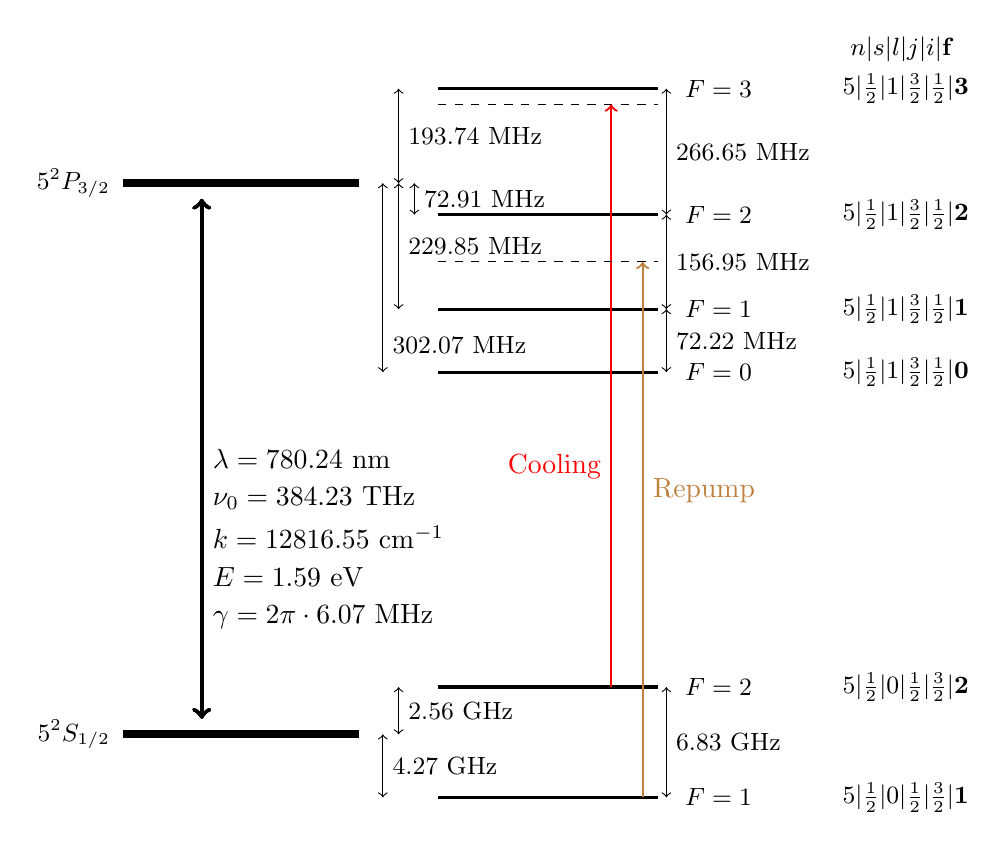
\begin{tikzpicture}[scale=2]

% lower level: 5s 1/2
\draw[line width=1mm] (-2.5,0) -- (-1,0) node[left, xshift=-3cm] {\small $5^2S_{1/2}$};
\draw[very thick] (-0.5,0.3) -- (0.9,0.3) node[right, xshift = 0.2cm] {\small $F = 2$};
\draw[very thick] (-0.5,-0.4) -- (0.9,-0.4) node[right, xshift = 0.2cm] {\small $F = 1$};

\draw[very thick] (-0.5,0.3) -- (0.9,0.3) node[right, xshift = 2.2cm] {\small $5 | \frac{1}{2} | 0 | \frac{1}{2} | \frac{3}{2} | \textbf{2}$};
\draw[very thick] (-0.5,-0.4) -- (0.9,-0.4) node[right, xshift = 2.2cm] {\small $5 | \frac{1}{2} | 0 | \frac{1}{2} | \frac{3}{2} | \textbf{1}$};

% annotate hfs for 5s: F=1 to F=2
\draw[<->] (0.95,0.3) -- (0.95,-0.4) node[midway,right] {\small $6.83~\text{GHz}$}; % 1 to 2

% annotate hfs for 5s: ground state to F=1,2
\draw[<->] (-0.85,0) -- (-0.85,-0.4) node[midway,right] {\small $4.27~\text{GHz}$}; % to 1
\draw[<->] (-0.75,0) -- (-0.75,0.3) node[midway,right] {\small $2.56~\text{GHz}$}; % to 2


% upper level: 5p 3/2
\draw[line width=1mm] (-2.5,3.5) -- (-1,3.5) node[left, xshift=-3cm] {\small $5^2P_{3/2}$};

\draw[very thick] (-0.5,4.1) -- (0.9,4.1) node[right, xshift = 0.2cm] {\small $F = 3$};
\draw[very thick] (-0.5,3.3) -- (0.9,3.3) node[right, xshift = 0.2cm] {\small $F = 2$};
\draw[very thick] (-0.5,2.7) -- (0.9,2.7) node[right, xshift = 0.2cm] {\small $F = 1$};
\draw[very thick] (-0.5,2.3) -- (0.9,2.3) node[right, xshift = 0.2cm] {\small $F = 0$};


\draw[very thick] (-0.5,4.1) -- (0.9,4.1) node[right, xshift = 2.3cm, yshift = 0.5cm] {\small $n | s | l | j | i | \textbf{f}$}; % extra annotation
\draw[very thick] (-0.5,4.1) -- (0.9,4.1) node[right, xshift = 2.2cm] {\small $5 | \frac{1}{2} | 1 | \frac{3}{2} | \frac{1}{2} | \textbf{3}$};
\draw[very thick] (-0.5,3.3) -- (0.9,3.3) node[right, xshift = 2.2cm] {\small $5 | \frac{1}{2} | 1 | \frac{3}{2} | \frac{1}{2} | \textbf{2}$};
\draw[very thick] (-0.5,2.7) -- (0.9,2.7) node[right, xshift = 2.2cm] {\small $5 | \frac{1}{2} | 1 | \frac{3}{2} | \frac{1}{2} | \textbf{1}$};
\draw[very thick] (-0.5,2.3) -- (0.9,2.3) node[right, xshift = 2.2cm] {\small $5 | \frac{1}{2} | 1 | \frac{3}{2} | \frac{1}{2} | \textbf{0}$};

% annotate hfs for 5p: each F state to other F state 
\draw[<->] (0.95,2.3) -- (0.95,2.7) node[midway,right] {\small $72.22~\text{MHz}$}; %0 to 1
\draw[<->] (0.95,2.7) -- (0.95,3.3) node[midway,right] {\small $156.95~\text{MHz}$}; % 1 to 2
\draw[<->] (0.95,3.3) -- (0.95,4.1) node[midway,right] {\small $266.65~\text{MHz}$}; % 2 to 3

% annotate hfs for 5p: ground state to each F state 
\draw[<->] (-0.85,3.5) -- (-0.85,2.3) node[below, right, yshift = 0.35cm] {\small $302.07~\text{MHz}$};
\draw[<->] (-0.75,3.5) -- (-0.75,2.7) node[midway,right] {\small $229.85~\text{MHz}$};
\draw[<->] (-0.65,3.5) -- (-0.65,3.3) node[midway,right] {\small $72.91~\text{MHz}$};
\draw[<->] (-0.75,3.5) -- (-0.75,4.1) node[midway,right] {\small $193.74~\text{MHz}$};


% cooling transition
\draw[dashed] (-0.5,4.0) -- (0.9,4.0) node[right] {};
% \draw[->,thick, color = red] (1,0.3) -- (1,4.0) node[midway, left, xshift=-0.2cm] {\small $780.241~\text{nm}$};
\draw[->,thick, color = red] (0.6,0.3) -- (0.6,4.0) node[midway, left, yshift = -0.9cm] {Cooling};


% repump transition
\draw[dashed] (-0.5,3.0) -- (0.9,3.0) node[right] {};
% \draw[->,thick, color = red] (1,0.3) -- (1,4.0) node[midway, left, xshift=-0.2cm] {\small $780.241~\text{nm}$};
\draw[->,thick, color = brown] (0.8,-0.4) -- (0.8,3.0) node[midway, right, yshift = 0.5cm] {Repump};



% annotate fs info
\draw[<->, line width = 0.5mm] (-2.0,0.1) -- (-2.0,3.4) node[midway,right, yshift = 0.0cm] {$\lambda = 780.24~\text{nm}$};
\draw[<->, line width = 0.5mm] (-2.0,0.1) -- (-2.0,3.4) node[midway,right, yshift = -0.5cm] {$\nu_0 = 384.23~\text{THz}$};
\draw[<->, line width = 0.5mm] (-2.0,0.1) -- (-2.0,3.4) node[midway,right, yshift = -1.0cm] {$k = 12816.55~\text{cm$^{-1}$}$};
\draw[<->, line width = 0.5mm] (-2.0,0.1) -- (-2.0,3.4) node[midway,right, yshift = -1.5cm] {$E = 1.59~\text{eV}$};
\draw[<->, line width = 0.5mm] (-2.0,0.1) -- (-2.0,3.4) node[midway,right, yshift = -2.0cm] {$\gamma = 2\pi \cdot 6.07~\text{MHz}$};



% \node at (1,-0.7) {\small $\lambda = 780.241209686(13)~\text{nm}$};
% \node at (1,-0.9) {\small $\nu = 384.2304844685(62)~\text{THz}$};
% \node at (1,-1.1) {\small $E = 1.589049439(58)~\text{eV}$};

\end{tikzpicture}

\end{document}
